\documentclass[12pt]{article}
\usepackage[utf8]{inputenc}
\usepackage[dvips]{graphicx}
\usepackage{epsfig}
\usepackage{verbatim}
\usepackage{array}
\usepackage{latexsym}
\usepackage{hyperref}
\usepackage{listings}
\usepackage{color}
\usepackage[hmargin=3cm,vmargin=5.0cm]{geometry}
\usepackage{tikz}
\usepackage{arydshln}
\usepackage{amssymb}



\topmargin=-1.8cm
\addtolength{\textheight}{6.5cm}
\addtolength{\textwidth}{2.0cm}
\setlength{\oddsidemargin}{0.0cm}
\setlength{\evensidemargin}{0.0cm}

\newcommand{\HRule}{\rule{\linewidth}{1mm}}

\usepackage{tikz}
\usetikzlibrary{trees}
\tikzset{
  font={\fontsize{7pt}{12}\selectfont}}
  
\newcommand{\Q}{\raisebox{1.7pt}{$\scriptstyle\bigcirc$}}

\lstset{
    %backgroundcolor=\color{lbcolor},
    tabsize=2,
    language=C++,
    basicstyle=\footnotesize,
    numberstyle=\footnotesize,
    aboveskip={0.0\baselineskip},
    belowskip={0.0\baselineskip},
    columns=fixed,
    showstringspaces=false,
    breaklines=true,
    prebreak=\raisebox{0ex}[0ex][0ex]{\ensuremath{\hookleftarrow}},
    %frame=single,
    showtabs=false,
    showspaces=false,
    showstringspaces=false,
    identifierstyle=\ttfamily,
    keywordstyle=\color[rgb]{0,0,1},
    commentstyle=\color[rgb]{0.133,0.545,0.133},
    stringstyle=\color[rgb]{0.627,0.126,0.941},
}

\usepackage[]{mdframed}
\usepackage{enumitem}

\usepackage{titlesec}
\titleformat{\subsection}[runin]{}{}{}{}[]









\begin{document}

% Set the overall layout of the tree
\tikzstyle{level 1}=[level distance=2.5cm, sibling distance=20em]
\tikzstyle{level 2}=[level distance=2.5cm, sibling distance=10em]

% Define styles for bags and leafs
\tikzstyle{bag} = [text width=16em, text centered, align=center]
\tikzstyle{end} = [circle, minimum width=3pt,fill, inner sep=0pt]

\noindent
\HRule \\[3mm]
\small
\begin{tabular}[b]{lp{4.3cm}r}
Middle East Technical University &  &
Department of Computer Engineering \\
\end{tabular} \\
\begin{center}

                 \LARGE \textbf{CENG 280} \\[4mm]
                 \Large Formal Languages and Abstract Machines \\[4mm]
                \normalsize Spring 2022-2023 \\
                    \Large Homework 2 \\
\end{center}
\HRule



% Write down your name, surname, and student ID below.
\begin{center}
Name Surname: Batuhan Akçan   \\
Student ID: 2580181
\end{center}



\section*{Answer for Q1}

\subsection*{a.} 
$ (a(b+c)^*a + b + aa)(a+b)^* $
\subsection*{b.}    \hfill\\
\textbf{A=}: 0       \newline
\textbf{B=}: 1       \newline
\textbf{C=}: 0,1       \newline
\textbf{D=}: 2       \newline
\textbf{E=}: 1       \newline
\textbf{F=}: 0,2       



\section*{Answer for Q2}
\subsection*{a.} 
State Elimination Algorithm
\subsection*{b.} 
\begin{itemize}
\item Step 1 should be modified. If the start state is an accepting state or has transitions in, we should add a new non-accepting state and add the transition $\epsilon/\epsilon$ between the new start state and the former start state. (Because we need to specify that the machine does not output anything while transitioning from the new start state and the former start state.)
\item Step 3 should be modified. After eliminating a state, we should update transitions for not only input symbols, but also output symbols. At the end, there will be only 1 state left, which is the start state that we have added. Also, there will be only 1 transition left, which is a loop in the start state, of the form REGEX1/REGEX2 (REGEX1 standing for input regular expression, REGEX2 standing for output regular expression).
\end{itemize}
\subsection*{c.}\hfill\vspace{0.5cm}\\

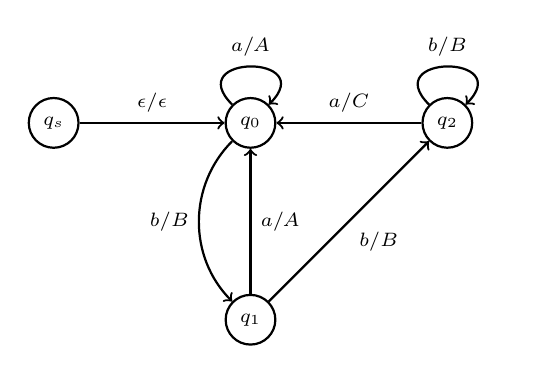
\begin{tikzpicture}[node distance={25mm}, thick, main/.style = {draw, circle}] 
\hspace{0cm}
\node[main] (1) {$q_s$}; 
\node[main] (2) [right of=1] {$q_0$}; 
\node[main] (3) [below of=2] {$q_1$}; 
\node[main] (4) [right of=2] {$q_2$};

\draw[->] (1) -- node[midway, above] {$\epsilon/\epsilon$} (2);
\draw[->] (2) to [out=135, in=45, looseness=5] node[midway, above] {$a/A$} (2);
\draw[->] (2) to [out=225, in=135] node[midway, left] {$b/B$} (3);
\draw[->] (3) -- node[midway, right] {$a/A$} (2);
\draw[->] (3) -- node[midway, below right] {$b/B$} (4);
\draw[->] (4) to [out=135, in=45, looseness=5] node[midway, above] {$b/B$} (4);
\draw[->] (4) -- node[midway, above] {$a/C$} (2);
\end{tikzpicture}\vspace{0.5cm}\\

\begin{tikzpicture}[node distance={25mm}, thick, main/.style = {draw, circle}] 
\node[main] (1) {$q_s$}; 
\node[main] (3) [below of=2] {$q_1$}; 
\node[main] (4) [right of=2] {$q_2$};

\draw[->] (1) to [out=270, in=180] node[midway, below left] {$a^*b/A^*B$} (3);
\draw[->] (3) to [out=225, in=315, looseness=5] node[midway, below] {$aa^*b/AA^*B$} (3);
\draw[->] (3) -- node[midway, below right] {$b/B$} (4);
\draw[->] (4) to [out=135, in=45, looseness=5] node[midway, above] {$b/B$} (4);
\draw[->] (4) to [out=180, in=90] node[midway, above left] {$aa^*b/CA^*B$} (3);
\end{tikzpicture}\vspace{0.5cm}\\

\begin{tikzpicture}[node distance={25mm}, thick, main/.style = {draw, circle}] 
\node[main] (1) {$q_s$};  
\node[main] (4) [right of=2] {$q_2$};

\draw[->] (1) -- node[midway, above] {$a^*b(aa^*b)^*b/A^*B(AA^*B)^*B$} (4);
\draw[->] (4) to [out=135, in=45, looseness=5] node[midway, above] {$b/B$} (4);
\draw[->] (4) to [out=270, in=270] node[midway, below] {$aa^*b(aa^*b)^*b/CA^*B(AA^*B)^*B$} (1);
\end{tikzpicture}\vspace{0.5cm}\\

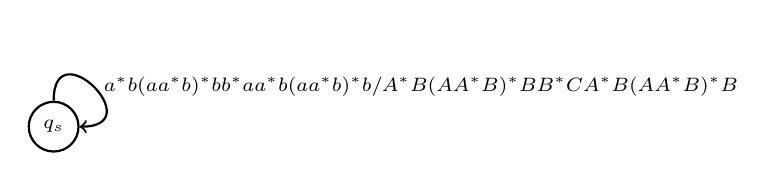
\begin{tikzpicture}[node distance={25mm}, thick, main/.style = {draw, circle}] 
\node[main] (1) {$q_s$};  

\draw[->] (1) to [out=90, in=0, looseness=5] node[midway, right] {$a^*b(aa^*b)^*bb^*aa^*b(aa^*b)^*b/A^*B(AA^*B)^*BB^*CA^*B(AA^*B)^*B$} (1);
\end{tikzpicture}\vspace{0.5cm}\\
Resultant set: $S = \{\; w \in O^* \; | $\;w ends with C\;$\} = \{\; w \in O^* \; | \; w = A^*B(AA^*B)^*BB^*C \;\}$\\
Regular expression: $A^*B(AA^*B)^*BB^*C$


\section*{Answer for Q3}
\begin{tikzpicture}



\end{tikzpicture}




\end{document}
